\section{Results}
\label{sec:results}

\begin{figure}[t]
  \centering
  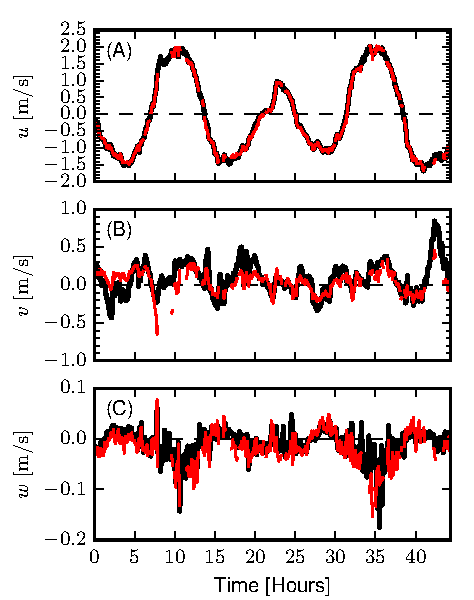
\includegraphics{TimeFig02}
  \caption{Time series of tidal velocity at Admiralty Head from ADV-IMU measurements (black), and an acoustic Doppler profiler on the anchor (red). The profiler measurements---taken at the same depth as the ADV on the TTM---were contaminated by acoustic reflection from the strongback fin when it was inline with one of the profiler's beams. Note that the vertical scale on the three axes vary by more than an order of magnitude; the small ticks in A and B are equivalent to the ticks in C.}
  \label{fig:vel_time}
\end{figure}

\subsection{Mean velocity}

Figure \ref{fig:vel_time} shows a comparison of $\vec{\bar u}$ measured by an ADV-IMU mounted on a TTM, to an upward-looking acoustic Doppler profiler mounted on the TTM anchor. This comparison shows excellent agreement between the ADV and Doppler profiler measurements of mean velocity. The $\bar u$, $\bar v$, and $\bar w$ components have a root-mean-square error of 0.05, 0.13, and 0.03 m/s, respectively. Although it is important to note that there is some discrepancy between ADP- and ADV-measured velocities (especially in $\bar v$, which is most likely due to incomplete motion correction), the agreement between the magnitude and direction of these independent velocity measurements indicates that moored ADV-IMUs provide a reliable estimate of mean velocity in the Earth's reference frame.

\subsection{TTM spectra}

\begin{figure*}[t]
  \centering
  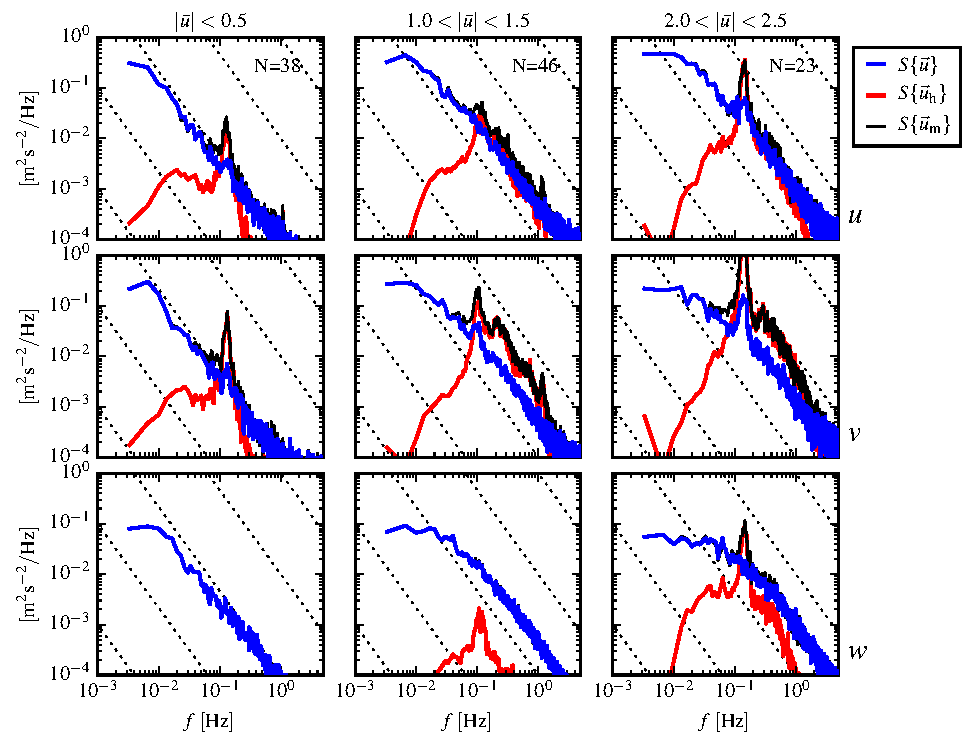
\includegraphics{SpecFig02_TTM02B-top}
  \caption{Turbulence spectra from the June 2014 TTM deployment. Each column is for a range of streamwise velocity magnitudes (indicated at top). The rows are for each component of velocity (indicated to the lower right of the right column). The uncorrected spectra are in black and the corrected spectra are blue, and the spectra of ADV head motion, $\uhead$, is red (also indicated in the legend). The vertical red dotted line indicates the filter frequency applied to the IMU accelerometers when estimating $\uhead$; below this frequency $\spec{\uhead}$ is plotted as a dashed line.   Diagonal black dotted lines indicate a $f^{-5/3}$ slope. The cyan line in the first and last rows indicates the semi-empirical Kaimal spectrum for the measured values of $\ustar$ and $U$. The number of spectral ensembles, N, in each column is indicated in the top row.}
  \label{fig:spec:ttm}
\end{figure*}

As discussed in detail in Part 1, the mooring motion of the TTM, $\spec{\uhead}$, has a peak at 0.1 to 0.2 Hz from swaying of the mooring that is most likely driven by eddy shedding from the spherical buoy (Figure \ref{fig:spec:ttm}, red lines). There is also higher-frequency broadband motion that is associated with fluttering of the strongback fin around the mooring line. Both of these motions are especially energetic in the $v$-component spectra because this is the direction in which the TTM mooring system is most unstable. As is expected from fluid-structure interaction theory, the amplitude of these motions increases with increasing mean velocity \cite[]{Morison++1950}.

The mooring motion contaminates the uncorrected ADV measurements of velocity, $\spec{\umeas}$, whenever the amplitude of the motion is similar to or greater than the amplitude of the turbulence. Fortunately, much of this motion can be removed using the IMU's motion signals as detailed in Section \ref{sec:methods}. Lacking an independent measurement of turbulence velocity at this site, we interpret the agreement of these spectra with turbulence theory as evidence that motion correction has improved the velocity measurements. In particular, at high frequencies ($f>0.3$ Hz) for each mean-flow speed, the spectra decay with a $f^{-5/3}$ slope and have equal amplitude across the velocity components. These results are consistent with \citeauthor{Kolmogorov1941c}'s (1941) theory of isotropic turbulence, and are consistent with the semi-empirical spectral form of \cite{Kaimal++1972}, and other earlier measurements of turbulence in energetic tidal channels from stationary platforms \cite[]{Walter++2011, Thomson++2012, McMillan++2016}.

The degree of agreement between Kaimal's theoretical form \cite[][]{Walter++2011}, and these measurements is encouraging, especially considering that $\ustar$ is estimated at the height of the measurement (10 m) rather than at the seafloor. This suggests that bottom-boundary layer physics are contributing to the turbulence at this site and depth, 10 m above the seafloor.

For $|\ue|>1.0$, motion correction modifies the $u$ and $v$ component spectra at frequencies as high as 3 Hz. This outcome indicates that in order for motion correction to be effective, synchronization between the ADV and IMU needs to be within 1/3 s or better. This suggests that asynchronous approaches to motion correction may be challenging, especially considering that the clock drift of some instrumentation can be as high as a few seconds per day. By integrating the IMU data into the ADV data stream, the Nortek ADV-IMU achieves a synchronization to within 1e-2 s. 

The low magnitude of $\spec{\uhead}$ at low frequencies is partially a result of filtering the IMU's accelerometer signal when calculating $\uacc$. The true low-frequency spectrum of ADV head motion is unknown (indicated using a dashed line below $f_a$). A comparison of $\spec{\ue}$ measured by the TTM to that measured by the ADP---during the June 2012 deployment---reveals agreement at low frequencies (not shown). This finding suggests that the assumption that $\ulow=0$ at these frequencies and at this site for this platform is justified---even if $\spec{\uhead}$ is not as low as indicated in Figure \ref{fig:spec:ttm}.

As successful as motion correction is, some of the motion contamination persists in $\spec{\ue}$. This is most notable in $\spec{v}$ at the highest flow speeds ($>2.0$ m/s): a peak at 0.15 Hz is an order of magnitude larger than a spectral fit to the other frequencies would indicate. This persistent motion contamination is evident to a lesser degree in $\spec{u}$ for $|u|>2$ m/s, and in $\spec{v}$ at lower flow speeds.  $\spec{w}$ appears to have no persistent motion contamination because the amplitude of the motion in this direction is much lower than for the other two components. For these measurements, $\spec{w_h}$ is so low that $w$-component motion correction makes only a minor correction to the spectra.

The amplitude of the persistent motion contamination peaks in $\spec{v}$ at 0.15 Hz is a factor of 5 to 10 times smaller than the amplitude of the ADV head motion itself. This observation suggests that the Microstrain IMU can be used to effectively correct mooring motion at 0.15 Hz when the amplitude of that motion is less than 5 times the amplitude of the real turbulence spectrum. As a result, we have chosen a value of 3 as a conservative estimate of the motion correction's effectiveness.

% Does this belong in the discussion?
In addition to the primary benefit of correcting for mooring motion, the IMU measurements can also be used to identify and screen out persistent motion contamination. For example, one of the most common uses of turbulence spectra is for the calculation of $\epsilon$ and $\tke$. For these purposes, and based on the relative amplitudes of the 0.15-Hz peaks, we assume that persistent motion contamination is likely, where $\spec{\uhead}/\spec{\ue} > 3$, and thereby exclude these regions from spectral fits.

In the present case, for the $u$ and $w$ spectra, this criteria only excludes a narrow range of frequencies at the 0.15-Hz motion peak for some cases. This criteria is more restrictive of the $v$-component spectra at high frequencies for $\bar U > 1.0$ m/s, but this may be acceptable because the amplitude of $\spec{v}$ at these frequencies---i.e., in the isotropic inertial subrange---should be equal to that of $\spec{u}$ and $\spec{w}$ \cite[]{Kolmogorov1941c}.

Agreement of the $v$-component spectral amplitude with that of $u$ and $w$ at frequencies $>0.3$ Hz indicates that motion correction is effective at those frequencies even when $\spec{\uhead}/\spec{\ue} \gtrsim 3$. This outcome suggests that our screening threshold is excessively conservative at those frequencies, and that a more precise screening threshold may be frequency dependent. For example, it might take into account the $~f^3$ character of the noise in $\spec{\uacc}$ (Figure \ref{fig:stnoise}). For the purpose of this work, the $\spec{\uhead}/\spec{\ue} < 3$ threshold for spectral fits is sufficient, and detailed characterization of the IMU's motion- and frequency-dependent noise level is left for future work.

\subsection{StableMoor Spectra}

\begin{figure*}[th]
  \centering
  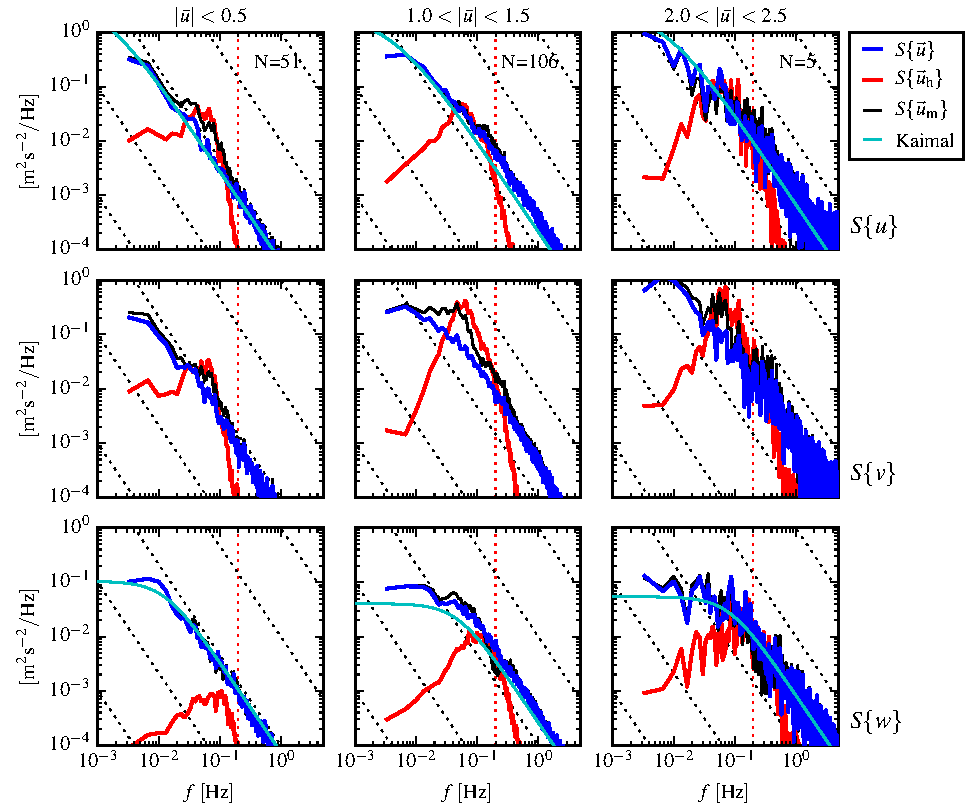
\includegraphics{SpecFig02_SMnose}
  \caption{Turbulence spectra from the StableMoor buoy. The axes layout and annotations are identical to Figure \ref{fig:spec:ttm}, except that $\spec{\uhead}$ is plotted as a solid line at all frequencies because it is measured at all frequencies. }
  \label{fig:spec:sm}
\end{figure*}

The spectra of the StableMoor motion has a broader peak with a maximum amplitude that is approximately half the frequency of the TTM spectral peak (Figure \ref{fig:spec:sm}). The motion of this platform also does not have high-frequency ``subpeaks" or other high-frequency broadbanded excitation (Part 1).  These characteristics of the motion are most likely due to the more massive and hydrodynamically streamlined properties of the platform. 

Like the TTM, the motion-corrected spectra from the StableMoor buoy are consistent with turbulence theory and previous observations. Most importantly, there is an improvement in the quality of the motion-corrected spectra compared to the TTM. In particular, the persistent motion contamination peaks are completely removed. That is, this measurement system provides an accurate estimate of the turbulence spectra at this location from low frequencies to more than 1 Hz---well into the inertial subrange---for all three components of velocity.

Note that this level of accuracy cannot be obtained without the independent estimate of $\ulow$. If we assume that $\ulow=0$, a similar plot to Figure \ref{fig:spec:sm} (not shown) reveals persistent motion-contamination peaks and troughs in the $u$ and $v$ spectra regardless of the choice of $f_a$. This assumption indicates that the low-frequency motion of the StableMoor buoy is below a threshold in which the IMU's signal-to-noise ratio is high enough to resolve its motion. In other words, compared to the TTM, the StableMoor platform provides a more accurate measurement of turbulence when it includes an independent measure of $\ulow$ (here a bottom-tracking ADCP), but it does no better---and perhaps worse---when it does not.
% * <sheri> 2016-10-21T00:00:00.000Z:
%
% Please define "ADCP" in the last sentence in the above paragraph - and put the acronym in parentheses after the definition.
%
% ^.


\subsection{Torpedo spectra}

\begin{figure}[t]
  \centering
  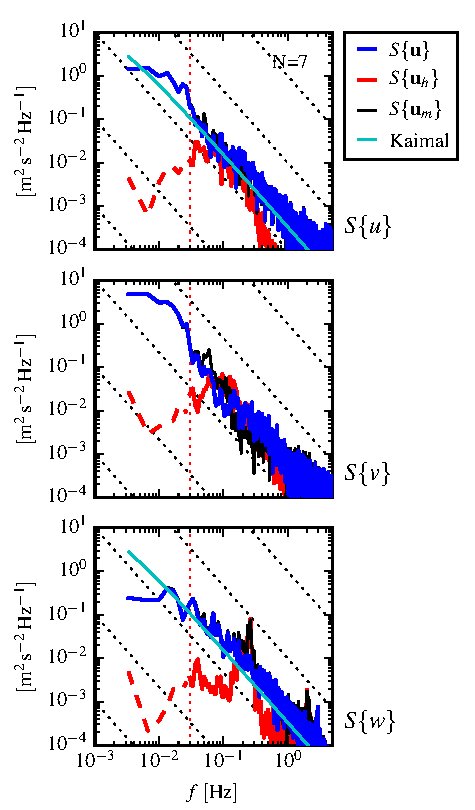
\includegraphics{SpecFig03_TTT}
  \caption{Turbulence spectra from the turbulence torpedo during a 35-minute period when the mean velocity was 1.3 m/s. Annotations and line colors are identical to Figure \ref{fig:spec:ttm}.}
  \label{fig:spec:torpedo}
\end{figure}

The $u$ and $v$ motion of the turbulence torpedo is broadband and the $w$ motion has a narrow peak at 0.3 Hz (Figure \ref{fig:spec:torpedo}). Because $\uhead$ is estimated using $f_a = 0.03$ Hz and assuming $\ulow=0$, its spectra rolls off quickly below $f_a$.  Motion correction of the torpedo data appears to effectively remove a motion peak from $\spec{w}$ at 0.3 Hz, and straightens out $\spec{v}$ between 0.04 and 0.6 Hz. $\spec{u}$ is mostly unaffected by motion at these frequencies, because the torpedo motion is smaller than the turbulence in this direction. At frequencies below $f_a$, $\spec{u}$ and $\spec{v}$ increase dramatically. This increase suggests that unresolved, low-frequency motion of the torpedo is contaminating the velocity measurements at these frequencies. It may be possible to correct for some of this contamination using a measurement of the ship's motion as a proxy for the torpedo's low-frequency motion, but this has not been done. Still, above $f_a$, the torpedo appears to provide a reliable estimate of spectral amplitude in the inertial subrange and can therefore be used to estimate $\epsilon$. Considering the simplicity of the platform, it may be a useful option for quantifying this turbulence statistic in a variety of scenarios. Further, if a GPS is positioned above it, it may be capable of providing even more.


\subsection{Cross Spectra}

\begin{figure*}[t]
  \centering
  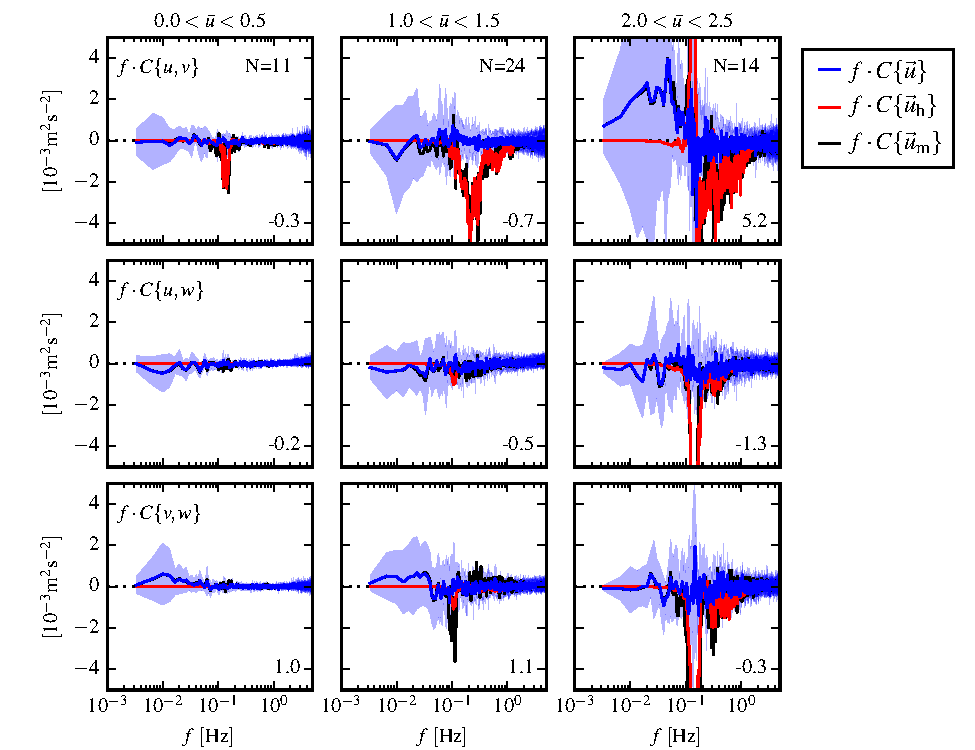
\includegraphics{StressSpec_TTM_03vp}
  \caption{Variance preserving cross-spectra between components of $\ue$ (blue), $\uhead$ (red), and $\umeas$ (black) from the June 2014 TTM deployment. The upper row is $f \cdot \cspec{u}{v}$, the middle row is $f \cdot \cspec{u}{w}$, and the bottom row is $f \cdot \cspec{v}{w}$.  Note that these cross-spectra are between components of a velocity vector (e.g., $\ue$), not between different vectors (i.e., not between $\ue$ and $\umeas$). The columns are for different ensemble-averages over distinct ranges of the stream-wise mean velocity magnitude (indicated above the top row). N is the number of spectral ensembles in each column. The light blue shading indicates one standard deviation of $f \cdot C\{\ue\}$. The number in the lower-right corner of each panel indicates the ensemble-averaged estimate of the Reynold's stress component (integral of the blue line) in units of  $\mathrm{10^{-3}\ m^2s^{-2}}$.}
  \label{fig:cspec:ttm}
\end{figure*}

Cross-spectra indicate the correlation between different velocity components as a function of frequency, and their integrals are the Reynold's stresses. Head motion cross-spectra, $C\{\uhead\}$ (Figure \ref{fig:cspec:ttm}, red), and uncorrected velocity cross-spectra, $C\{\umeas\}$ (black), from TTM measurements have large peaks at the same frequency (~0.15 Hz) as peaks in auto-spectra (Figure \ref{fig:spec:ttm}).  This indicates that mooring motion contaminates the uncorrected cross-spectral velocity measurements, and that Reynold's stress estimates based on uncorrected velocity measurements will be contaminated by mooring motion. This makes sense because mooring swaying in a direction not aligned with one of the major principal axes will, for example, introduce spurious cross-spectra and contaminate the Reynold's stress.

Fortunately, motion corrected velocity cross-spectra, $C\{\ue\}$ (blue), have reduced spectral amplitudes at these frequencies (reduced peaks), which indicates that motion correction reduces motion contamination to produce more reliable estimates of velocity cross spectra and Reynold's stresses (Figure \ref{fig:cspec:ttm}). In particular, the uncertainty in $f\cdot C\{\ue\}$ (indicated by the blue shading), is significantly smaller than the mean values of $C\{\uhead\}$ and $C\{\umeas\}$ at the frequencies of maximum motion (0.15 Hz). This indicates that even the individual values of $C\{\ue\}$ are reduced at these frequencies, compared to $C\{\umeas\}$, not just their mean. 

% Still, care should be taken when interpreting 

% At low flow speeds (left column), cross spectra between components of $\uhead$ (i.e., between components of head motion, red) are small compared to correlated velocities. As the velocity magnitude increases (center and right columns), the swaying motion of the TTM at 0.15 Hz appears as a peak in the amplitude of the cross spectra of $\uhead$ (red) and $\umeas$ (black) for all three components of cross spectra (rows). Fortunately, motion correction reduces the amplitude of this peak dramatically so that $C\{\ue\}$ (blue) is small at 0.15 Hz compared to lower frequencies. Furthermore, the fact that the standard deviation of $C\{\ue\}$ is also relatively small at 0.15 Hz suggests that motion correction is effective for each spectral window, not just in their mean.

These results indicate that motion-corrected TTM velocity measurements can be used to estimate turbulence Reynold's stresses, which are the integral of the cross spectra. Without motion correction, Reynold's stress estimates would be contaminated by the large peaks in the cross spectra that are caused by the swaying and fluttering motion of the TTM vane.

A similar investigation of StableMoor cross spectra (not shown) indicates that cross-spectral motion contamination is at a much lower amplitude than for the TTM. The low-frequency ($<0.3$ Hz) ``swimming'' motion of that platform produces a minimal cross-spectral signal, and the relative large mass of the platform minimizes the kinds of higher-frequency swaying and fluttering that creates large values of cross-spectral head motion. Thus, the StableMoor platform also produces reliable estimates of Reynold's stresses, which are presumed to be improved by motion correction. However, because the StableMoor is less-stable in pitch than the TTM (see Part I for details), the TTM has lower noise in it's $\uw$ estimates than the StableMoor.

%\section{Other stuff}




%%% Local Variables:
%%% mode: latex
%%% TeX-master: "Kilcher_etal_IMU-ADV"
%%% End:
